\section{Background}
\subsection{Frequency and Time Period}
\label{sec:fAndT}
\textbf{Frequency} is defined as the number of occurrences of a periodic event per unit time \parencite[78]{allum2023}. \textbf{Time period} is referred to as the amount of time between each iteration of an event which happens periodically \parencite[78]{allum2023}. These two terms stand in an inverse relationship
\begin{equation}
	f = \frac{1}{T}
	\label{eq:fAndT}
\end{equation}
where $f$ is frequency in $Hz$ and $T$ is time period in seconds. This relationship is later utilized to extrapolate the vortex shedding frequency in both the theoretical and the practical investigation.
\subsection{Fundamentals of Fluid Dynamics}
The definition of vorticity, a vortex and a bluff body must be understood. \textbf{Vorticity} is the vector quantity representing the rotational motion in a velocity field \parencite[p.~2500]{holton2003_vorticity}. A \textbf{vortex} is the circular flow of a fluid around a central axis, characterized by the vorticity in the fluid \parencite[p.~390]{nitsche2006_vortex}. A \textbf{bluff body} is defined as an object that, due to its geometry, induces significant regions of separated flow \parencite[p.~561]{navalhydro1997}. 

Furthermore, one must distinguish between a Newtonian and a non-Newtonian fluid. A \textbf{Newtonian fluid} is a fluid in which the viscosity \textemdash\ a measure of internal friction \textemdash\ remains constant despite applied shear rate, whereas a \textbf{non-Newtonian} fluid exhibits a viscosity which varies with the applied force \parencite{mohn2024}. 

Moreover, one must also consider the type of flow. There are two key factors of flow when investigating vortex shedding: laminar and turbulent flow, and compressible and incompressible flow. \textbf{Laminar flow} is characterized by the layered motion of fluid particles, with no significant disturbance between the parallel layers \parencite[pp.~40--41]{versteeg2007}. On the other hand, \textbf{turbulent flow} is known to have continuous, irregular fluctuations in velocity and pressure throughout the fluid \parencite[p.~40]{versteeg2007}. A \textbf{compressible flow} is a flow in which the fluid does not have a uniform density \parencite[p.~31]{oran2002}, conversely, an \textbf{incompressible flow} is a flow in which the fluid has a constant density \parencite[p.~12]{versteeg2007}. 

Lastly, two dimensionless numbers must be considered: the Reynolds and Strouhal number. The \textbf{Reynolds number} expresses the “ratio between inertial and viscous forces” \parencite{nasa_reynolds, noauthor_relationship_nodate}. Given by the equation 
\begin{equation}
	\mathrm{Re} = \frac{U L}{\nu}
	\label{eq:reynoldsNumber}
\end{equation}
where $U$ is the free-stream velocity ($m\,s^{-1}$), $L$ is the characteristic length ($m$) and $\nu$ is the kinematic viscosity ($m^2\,s^{-1}$). This number allows one to classify if a flow is laminar or turbulent, with low Reynolds numbers signifying laminar flow and high Reynolds number indicating turbulent flow \parencite{saldana2024_reynolds}. The \textbf{Strouhal number} is a dimensionless parameter used to describe the periodicity of vortex shedding \parencite[p.~211]{choi2000strouhal}. It is given by the equation 
\begin{equation}
	\mathrm{St} = \frac{f L}{U}
	\label{eq:strouhalNumber}
\end{equation}
where $f$ is the frequency of vortex shedding ($Hz$), $L$ is the characteristic length ($m$) and $U$ is the free-stream velocity ($m\,s^{-1}$). A high Strouhal number \textemdash\ assuming both $L$ and $U$ remain constant \textemdash\ indicates an increased vortex shedding frequency $f$, conversely a low Strouhal number indicates a lower $f$.

This essay will analyze vortex shedding in a Newtonian fluid \textemdash\ water \textemdash\ which exhibits laminar and incompressible flow. A Reynolds number of 100 was targeted in order to ensure laminar flow \parencite[2]{alammar_wake_nodate}; however, due to practical limitations, this was only fully realized theoretically and not in practice \textemdash\ details of which are discussed later.

\subsection{Vortex Shedding and the Kármán Vortex Street}
Vortex shedding in a two-dimensional plane can be defined as the phenomenon in which localized regions of high vorticity are periodically released into the wake from alternating sides of a bluff body, each exhibiting an opposite rotational direction \parencite[156]{green1995fluid}. Whereas vortex shedding is the process by which vortices are formed, Kármán Vortex Street refers to the flow pattern created, a repeated structure of counter-rotating vortices \parencite[26]{govardhan2005karman}.

\begin{figure}[htbp]
	\centering
	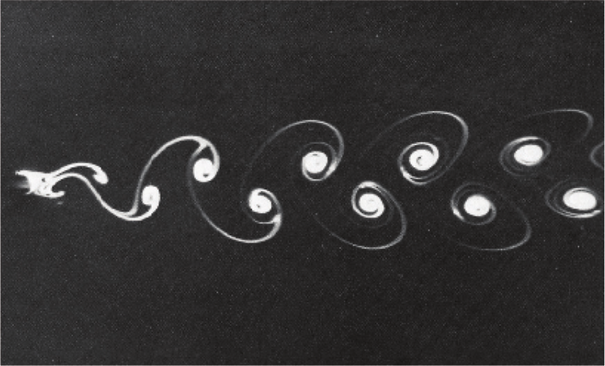
\includegraphics[width=0.7\textwidth]{images/vonKarmanStreet.png}
	\caption{Von Kármán Street behind a cylinder in a non-rotating 2D flow for Re = 140, fluorescein visualization \parencite[144]{ilieva2017turbulence}}
	\label{fig:vonKarmanStreet}
\end{figure}
\subsection{The Mechanism of Vortex Shedding}
Due to the fiction between a given fluid and a bluff body, there is no relative motion between them \parencite{boundaryLayerTheory_2018, jeff_defoe_bluff_2020}. Consequently, if the velocity of the bluff body is zero, the velocity of the fluid at the wall of the bluff body, with respect to the reference frame of the bluff body, is also zero: a no-slip condition. This causes a variation in velocities with distance, from zero at the bluff body surface to the free stream velocity U at a certain distance from the bluff body. The region in which this velocity gradient occurs is referred to as the boundary layer.

\pgfdeclarelayer{background}
\pgfdeclarelayer{foreground}
\pgfsetlayers{background,main,foreground}

\begin{figure}[H]
	\begin{center}
		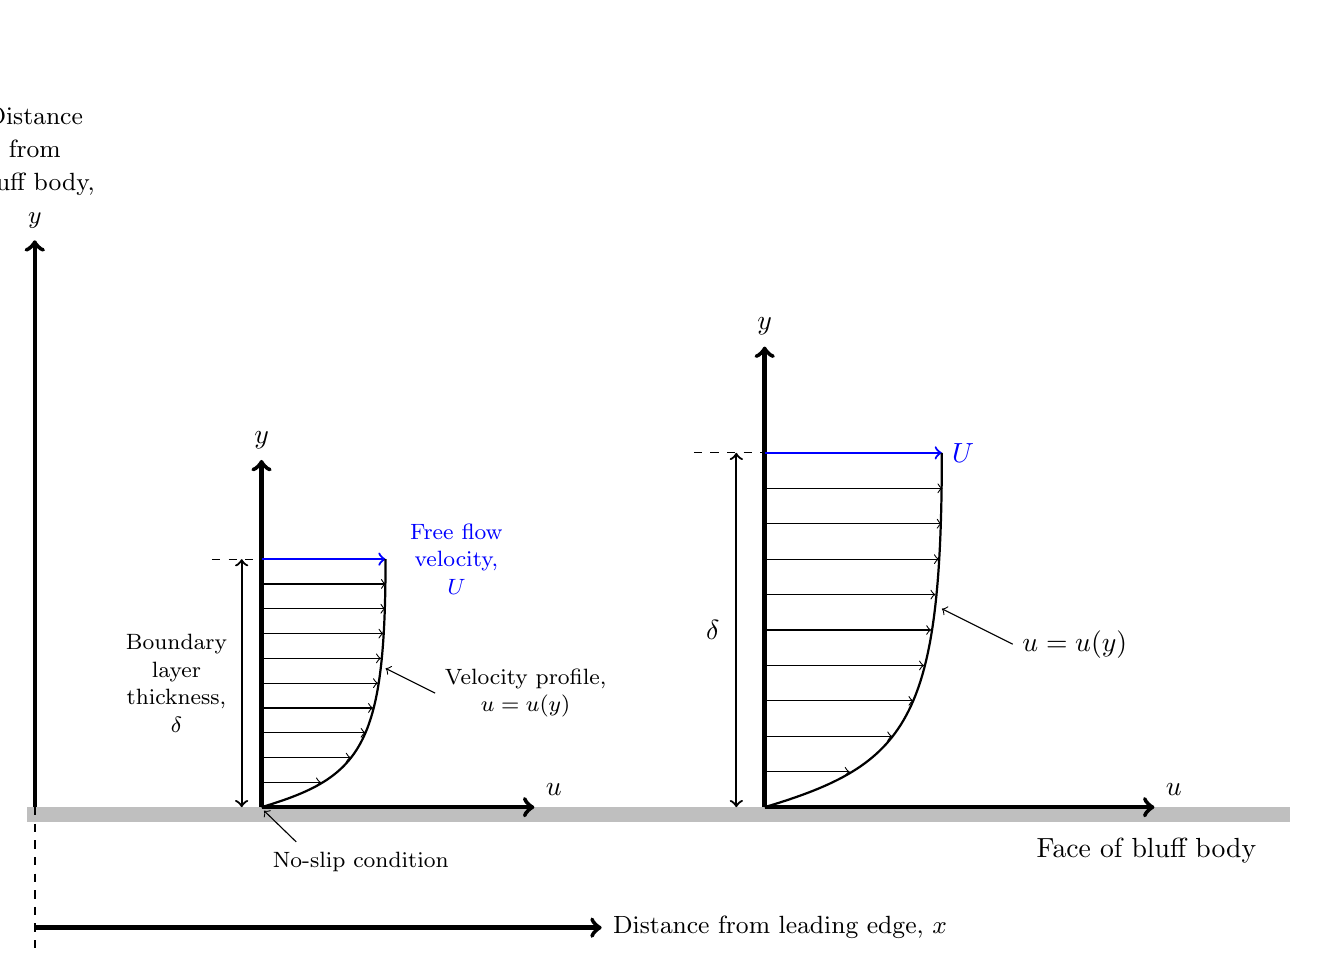
\begin{tikzpicture}[scale=0.9]
			\path[use as bounding box] (-7.1,0) rectangle (10.7,13);
			
			\begin{scope}[shift={(0, 2)}]
				\draw[->, ultra thick] (-7,0) -- (-7,8) node[above, align=center] {\small Distance \\ \small  from \\ \small  bluff body, \\ \small  $y$};
				\draw[dashed, thick] (-7,0) -- (-7, -2);
				\draw[->, ultra thick] (-7, -1.7) -- (1, -1.7) node[right] {\small  Distance from leading edge, $x$};
				
				% Wall
				\begin{pgfonlayer}{background}
					\filldraw[lightgray] (-7.1,-0.2) rectangle (10.7, 0);
					\node[anchor=north west] at (7, -0.3) {Face of bluff body};
				\end{pgfonlayer}
				
				\begin{scope}[shift={(-3.8,0)}, scale=0.7]
					% Axes
					\draw[->, ultra thick] (0,0) -- (0,7) node[above] {$y$};
					\draw[->, ultra thick] (0,0) -- (5.5,0) node[above right] {$u$};
					
					\node[anchor=north] at (2, -0.7) {\footnotesize No-slip condition};
					\draw[->, anchor=north] (0.7, -0.7) -- (0.05, -0.07);
					
					% Boundary layer thickness
					\draw[dashed] (-1,5) -- (2.5,5);
					\draw[<->, thick] (-0.4,0) -- (-0.4,5);
					\node[anchor=east, align=center] at (-0.5,2.5) {\footnotesize Boundary\\[-0.2em] \footnotesize layer\\[-0.2em] \footnotesize thickness,\\[-0.2em] {\footnotesize$\delta$}};
					
					
					% External flow
					\draw[->, thick, blue] (0,5) -- (2.5,5);
					\node[blue, anchor=west, align=center] at (2.8,5) {\footnotesize Free flow\\[-0.2em] \footnotesize velocity,\\[-0.2em] \footnotesize$U$};
					
					% Curve
					\draw[thick](0,0)
					.. controls (2, 0.6) and (2.5, 1.2) .. (2.5, 5); 
					
					% Arrows
					\draw[->] (0,0.5) -- (1.2, 0.5);
					\draw[->] (0,1) -- (1.8, 1);
					\draw[->] (0, 1.5) -- (2.1, 1.5);
					\draw[->] (0,2) -- (2.25, 2);
					\draw[->] (0, 2.5) -- (2.35, 2.5);
					\draw[->] (0,3) -- (2.41, 3);
					\draw[->] (0, 3.5) -- (2.46, 3.5);
					\draw[->] (0,4) -- (2.5, 4);
					\draw[->] (0, 4.5) -- (2.51, 4.5);
					
					% Velocity profile label
					\node[anchor=west, align=center] at (3.5,2.3) {\footnotesize Velocity profile, \\[-0.2em] \footnotesize$u = u(y)$};
					\node[anchor=west] at (3.5,1.8) {};
					\draw[->, anchor=east] (3.5, 2.3) -- (2.5, 2.8);
				\end{scope}
				
				\begin{scope}[shift={(3.3,0)}]
					% Axes
					\draw[->, ultra thick] (0,0) -- (0,6.5) node[above] {$y$};
					\begin{pgfonlayer}{foreground}
						\draw[->, ultra thick] (0,0) -- (5.5,0) node[above right] {$u$};
					\end{pgfonlayer}
					
					
					% Boundary layer thickness
					\draw[dashed] (-1,5) -- (2.5,5);
					\draw[<->, thick] (-0.4,0) -- (-0.4,5);
					\node[anchor=east] at (-0.5,2.5) {$\delta$};
					
					% External flow
					\draw[->, thick, blue] (0,5) -- (2.5,5);
					\node[blue] at (2.8,5) {$U$};
					
					% Curve
					\draw[thick](0,0)
					.. controls (2, 0.6) and (2.5, 1.2) .. (2.5, 5); 
					
					% Arrows
					\draw[->] (0,0.5) -- (1.2, 0.5);
					\draw[->] (0,1) -- (1.8, 1);
					\draw[->] (0, 1.5) -- (2.1, 1.5);
					\draw[->] (0,2) -- (2.25, 2);
					\draw[->] (0, 2.5) -- (2.35, 2.5);
					\draw[->] (0,3) -- (2.41, 3);
					\draw[->] (0, 3.5) -- (2.46, 3.5);
					\draw[->] (0,4) -- (2.5, 4);
					\draw[->] (0, 4.5) -- (2.51, 4.5);
					
					% Velocity profile label
					\node[anchor=west] at (3.5,2.3) {$u = u(y)$};
					\draw[->, anchor=east] (3.5, 2.3) -- (2.5, 2.8);
				\end{scope}
			\end{scope}
			
			
		\end{tikzpicture}
	\end{center}
	\caption{Depiction of boundary layer and the velocity gradient formed. Inspired by \textcite{erau_boundarylayer}}
	\label{fig:boundaryLayer}
\end{figure}

When a flow moves past a bluff body in a two-dimensional plane, a boundary layer develops, with increasing thickness $\delta$ from the stagnation point \parencite{fitzpatrick2016_reynolds}, the point on the leading edge of the bluff body at which the local fluid velocity is zero (with respect to the bluff body), to the back of the bluff body \parencite{learneng2022_boundarylayer}. At a certain point, the boundary layer separates from the bluff body, forming a shear layer. Under steady flow conditions, this separation occurs in a periodic and alternating manner, creating two separate, out-of-phase shear layers on either side of the bluff body. 

\begin{figure}[H]
	\begin{center}
		\begin{tikzpicture}[scale=0.2, >=Stealth]
			
			% Main vertical flow arrow
			\draw[->, thick] (0,39) -- (0,36) node[midway, right] {Flow};
			
			% Obstacle rectangle
			\draw[pattern=north east lines, pattern color=black!50] (-4,33) rectangle (4,30);
			
			% Shear layers 
			\draw (-4, 33)
			.. controls (-5, 32) and (-4.7, 25) .. (-4.7, 23);
			\draw (-4.7, 23)
			.. controls (-4.5, 21) and (-4, 19) .. (-2, 17);
			\draw (-2,17)
			.. controls (-1.5, 16.5) and (0, 15.5) .. (-2, 14.8);
			\draw (-2, 14.8)
			.. controls (-5, 14) and (-7.8, 12) .. (-8.6, 5);
			\draw (-8.6, 5)
			.. controls (-8.7, 4) and (-8.9, 1) .. (-6.8, -3);
			
			
			\draw (-4, 30)
			.. controls (-4, 27) and (-3.7, 25) .. (-3.7, 23);
			\draw (-3.7, 23)
			.. controls (-3.5, 21) and (-2, 19) .. (-1, 18);
			\draw (-1,18)
			.. controls (-0.5, 17.5) and (0, 17) .. (0.5, 17.5);
			\draw (0.5, 17.5)
			.. controls (1, 18) and (2, 20) .. (2.2, 22);
			\draw (2.2, 22)
			.. controls (2, 24) and (2, 25) .. (0.9, 27.41);
			
			
			\begin{scope}[shift={(-0.3,7.9)}]
				\draw (1.24,19.55) -- (0.75 ,19.125) -- (0.8,21) -- (2.25,20.25) -- (1.65,19.8);
			\end{scope}
			
			
			\draw (2, 17.5)
			.. controls (2.3, 18) and (3, 20) .. (3, 22);
			\draw (3, 22)
			.. controls (2.7, 24) and (2.7, 25) .. (1.4, 27.7);
			
			
			\draw (2, 17.5)
			.. controls (1.3, 16.5) and (1.5, 16) .. (2, 15.9);
			
			
			\draw (2, 15.9) -- (3, 15.7);
			
			
			\draw (3, 15.7) -- (3, 16.5) -- (4.3, 15.4) -- (3, 14.3) -- (3, 15.1);
			
			
			\draw (3, 15.1)
			.. controls (2.5, 15) and (2.1, 15) .. (1.8, 14.6);
			
			
			\draw (1.8, 14.6)
			.. controls (1.1, 14) and (3, 13) .. (3.5, 9);
			
			
			\draw (3.5, 9) -- (4.1, 9) -- (3.1, 7.7) -- (2, 9) -- (2.7, 9);
			
			
			\draw (2.7, 9)
			.. controls (3, 9.7) and (2.5, 12.5) .. (0, 13.6);
			\draw (0, 13.6)
			.. controls (-0.3, 13.8) and (-1, 13.8) .. (-1, 13.8);
			
			
			\draw (-1, 13.8)
			.. controls (-6.4, 13.5) and (-7, 9) .. (-7.5, 7.5);
			\draw (-7.5, 7.5)
			.. controls (-7.8, 6) and (-8, 4) .. (-7.9, 3);
			\draw (-7.9, 3)
			.. controls (-7.6, 1) and (-7.35, 0) .. (-6.25, -2.6);
			\draw (-6.8, -3) -- (-6.25, -2.6);
			
			
			
			\draw (4, 33)
			.. controls (4.5, 32) and (5, 25) .. (5.7, 23);
			\draw (5.7, 23)
			.. controls (7.5, 15) and (7, 10) .. (5.6, 5);
			\draw (5.6, 5)
			.. controls (4.8, 3) and (3.7, 2) .. (2, 1.3);
			\draw (2, 1.3)
			.. controls (0, 0.7) and (-1, 1) .. (-2, 1.2);
			\draw (-2, 1.2)
			.. controls (-7, 3) and (-6, 8) .. (-5.3, 9.5);
			\draw (-5.3, 9.5)
			.. controls (-4.5, 12) and (-1.8, 13.2) .. (0, 12.3);
			\draw(0, 12.3)
			.. controls (1.5, 11.5) and (2.5, 9) .. (0, 7);
			
			\draw (4, 30)
			.. controls (4, 30) and (4.3, 25) .. (4.7, 23);
			\draw (4.7, 23)
			.. controls (6, 15) and (6, 10) .. (4.2, 5);
			\draw (4.2, 5)
			.. controls (3.7, 3.8) and (2.7, 3) .. (1.8, 2.6);
			\draw (1.8, 2.6)
			.. controls (-1, 1.8) and (-2.7, 2.4) .. (-4, 4.8);
			\draw (-4, 4.8)
			.. controls (-5.2, 7) and (-4.2, 9) .. (-3.5, 10);
			\draw (-3.5, 10)
			.. controls (-3, 10.5) and (-2, 12) .. (0, 10.7);
			\draw(0, 10.7)
			.. controls (0.5, 10) and (0.9, 9.3) .. (0, 7);
			
			\node[anchor=west] at (6.9,26) {Flow C};
			\draw[->] (6.9, 26) -- (2.5, 23);
			
			\node[anchor=west] at (9,32) {Formation Region};
			\draw[->] (9, 32) -- (3, 28.5);
			
			\node[anchor=west] at (8,13.5) {Flow B};
			\draw[->] (8, 13.5) -- (2.5, 15.5);
			
			\node[anchor=west] at (7.5,6.5) {Flow A};
			\draw[->] (7.5, 6.5) -- (2.8, 11);
			
			\node[anchor=east] at (-8,25) {Shear layer $SL_2$};
			\draw[->] (-8, 25) -- (-4, 22);
			
			\node[anchor=west] at (10,20.5) {Shear layer $SL_1$};
			\draw[->] (10, 20.5) -- (5.9, 19);
			
			\node[anchor=north] at (0,-6.5) {Wake axis};
			
			\node[anchor=west] at (10,-1) {Growing vortex $V_1$};
			\draw[->] (10, -0.5) -- (-2, 7);
			
			% Wake axis dashed line
			\draw[dashed] (0,35) -- (0,-6.5);
			
		\end{tikzpicture}
	\end{center}
	\caption{The mechanism of vortex shedding. Inspired by \textcite[3]{shen2010_vortexmeter}}
	\label{fig:mechanismOfVortexShedding}
\end{figure}

For simplification, assume the first shear layer is generated at the right of the bluff body ($SL_{1}$). Due to its vorticity, the shear layer tends to curl up, forming a vortex. As the vortex forms, the pressure in the core of the vortex decreases, acting as a sink, inducing inflow towards its center. The fluid initially present at the bottom of the backside of the bluff body is drawn into the vortex, creating space, allowing for the formation of the left shear layer ($SL_{2}$) in the \textit{formation region}. This newly created shear layer splits into three distinct flows: a flow (\textit{Flow C}) which recirculates behind the bluff body, a flow (\textit{Flow B}) which mixes with the top shear layer and a flow (\textit{Flow A}) which is drawn into the vortex ($V_{1}$).

There is a decrease in strength of the vortex being created due to \textit{Flow A} having an opposite vorticity to the vorticity of the vortex. Moreover, the opposite vorticity of \textit{Flow B} and the right shear layer effectively nullifies each other, leading to the right shear layer being interrupted and the vortex becoming detached, causing it to travel with the main flow. The vortex has been “shed”. Since the vortex moves away from the bluff body, its low-pressure influence on the area near the bluff body decreases, allowing the left shear layer to more freely develop. Now, due to the periodic nature of vortex formation, the process recurs with the shear layers switching roles. 

When considering the vortex being created from the top shear layer, the fluid at the top of the vortex will have the same velocity as the free stream velocity U, whereas the velocity at the bottom of the vortex will be of a smaller magnitude and in the opposite direction of the main flow. According to Bernoulli’s equation, a region of higher velocity must have a lower pressure and vice versa. Therefore, the bottom region of the vortex will have a higher pressure than the top region, causing a lift force which acts on the bluff body normal to the flow. The oscillation of this lift force coincides with the vortex shedding frequency $f$, the frequency at which the vortices are alternately shed from opposite sides of the bluff body. 

\subsection{Hypothesis}
It is hypothesized that as the number of faces of the bluff body increases from 2 to 12, the vortex shedding frequency in laminar flow will decrease. This trend is attributed to a decrease in the Strouhal number, as shown by \textcite{goncalves1999strouhal}, which is directly proportional to the vortex shedding frequency, as seen in Equation \eqref{eq:strouhalNumber}. 




